\documentclass[10pt,a4paper]{article}
\usepackage{mathtools}
\usepackage[T1]{fontenc}
\usepackage{lmodern}
\usepackage{textcomp}

\usepackage[english]{babel}

\usepackage{amsmath, amssymb}

\usepackage{booktabs}
\usepackage{graphicx}
\usepackage[font=small,labelfont=bf,labelsep=period,tableposition=top]{caption}
\usepackage[T1]{fontenc}
\usepackage[utf8]{inputenc}
\usepackage{amsthm}
\usepackage[]{algorithm2e}
\usepackage{xcolor}
\usepackage{listings}



\title{Modelli probabilistici per le decisioni: SmartHouse}
\author{Matteo Angelo Costantini, matricola: 795125 \\
	Alessandro Longhi, matricola: 794235}
\date{}
\begin{document}
	\maketitle
	\clearpage
	\tableofcontents
	\clearpage
	\section{Introduzione}
	I miglioramenti ottenuti in ambito medico hanno portato ad un sensibile aumento dell'aspettativa di vita di ogni individuo, causando un generale invecchiamento della popolazione; il quale rappresenta un importante argomento di studi nell'ambito della sanità. Infatti, aumentando il numero di individui anziani, aumenta anche la necessità di studiare e trovare una soluzione ad alcuni problemi associati alla vecchiaia.
	
	Focalizzarsi sui problemi dovuti all'anzianità significa, quindi, trovare dei modi efficienti per fornire supporto e cure agli individui più anziani direttamente a casa loro; tutto ciò è reso possibile grazie all'uso di sistemi di monitoraggio all'interno delle case, in quanto permettono sia l'aumento della sicurezza dell'abitante, sia il senso di protezione di quest'ultimo, favorendone l'autonomia.
	
	Monitorare le azioni quotidiane degli individui è uno dei task più importanti all'interno di quest'ambito, in quanto permette di descrivere il benessere degli abitanti delle case, sia fisico che mentale. Il monitoraggio delle attività avviene grazie all'uso di alcuni sensori, i quali vengono posti in diversi luoghi all'interno di ogni abitazione. 
	
	Questo progetto si colloca nell'ambito appena descritto: avendo a disposizione dei dataset contenenti le rilevazioni delle attività e dei sensori in due abitazioni differenti, il lavoro svolto consiste nella definizione di un modello HMM in grado di inferire le attività data una sequenza di osservazioni derivanti dai sensori. Una volta creata la struttuta HMM, è stata effettuata un'analisi riguardante la capacità predittiva del modello.
	
	(INSERIRE LA STRUTTURA DELLA RELAZIONE CHE SEGUIRA). 
	
	
	\clearpage
	\section{Analisi del dataset}
	I dataset a nostra disposizione erano quattro, due per ogni abitazione, rappresentanti rispettivamente le attività ed i sensori rilevati all'interno dell'abitazione.
	
	Le abitazioni considerate sono due, etichettate con "OrdonezA" ed "OrdonezB".
	\subsection{Analisi del dataset A}
	Per l'abitazione "OrdonezA" sono stati forniti due dataset: uno denominato "OrdonezA\_ADLs" contenente le attività rilevate, ed uno denominato "OrdonezA\_Sensors" contenente i sensori rilevati.
	Nel primo dataset, quello delle attività, sono descritti i seguenti campi:
	\begin{itemize}
		\item Start\_time: data ed ora di inizio della rilevazione di un'attività
		\item End\_time: data ed ora di fine della rilevazione di un'attività
		\item  Activity: attività rilevata nel periodo considerato
	\end{itemize}
	
	in particolare, nella colonna "Activity" sono stati rilevati 10 valori diversi, cioè: Leaving, Toileting, Showering, Sleeping, Breakfast, Lunch, Dinner, Snack, Spare\_Time/TV e Grooming. 
	
	Il secondo dataset di "OrdonezA"è dedicato alla raccolta dei sensori rilevati. In quest'ultimo sono presenti i seguenti campi:
	\begin{itemize}
		\item Start\_time: data ed ora di inizio della rilevazione di un sensore
		\item End\_time: data ed ora di fine della rilevazione di un sensore
		\item  Location: collocazione precisa in cui è posizionato il sensore rilevato
		\item Type: tipologia del sensore rilevato
		\item Place: camera dell'abitazione nella quale è posizionato il sensore rilevato
	\end{itemize}
	
	in particolare, nella colonna "location" sono stati rilevati 12 sensori in 4 camere diverse, che, divisi in base al tipo, sono:
	
	\begin{itemize}
		\item tipo PIR: Shower, Basin, Cooktop
		\item tipo Magnetic: Maindoor, Fridge, Cabinet, Cupboard
		\item  tipo Flush: Toilet
		\item tipo Pressure: Seat, Bed
		\item tipo Electric: Microwave, Toaster
	\end{itemize}
	
	Per entrambi i dataset di A, sono state considerate le rilevazioni ottenute per un periodo di 14 giorni, dal 28-11-2011 al 11-12-2011.
	
	\subsection{Analisi del dataset B}
	
	Per l'abitazione "OrdonezB" sono stati forniti due dataset: uno denominato "OrdonezB\_ADLs" contenente le attività rilevate, ed uno denominato  "OrdonezB\_Sensors"	 contenente i sensori rilevati.
	
	Nel primo dataset, quello delle attività, sono descritti i seguenti campi:
	
	\begin{itemize}
		\item Start\_time: data ed ora di inizio della rilevazione di un'attività
		\item End\_time: data ed ora di fine della rilevazione di un'attività
		\item  Activity: attività rilevata nel periodo considerato
	\end{itemize}
	
	in particolare, nella colonna "Activity" sono stati rilevati 10 valori diversi, cioè: Leaving, Toileting, Showering, Sleeping, Breakfast, Lunch, Dinner, Snack, Spare\_Time/TV e Grooming. 
	
	Il secondo dataset di "OrdonezB"è dedicato alla raccolta dei sensori rilevati. In quest'ultimo sono presenti i seguenti campi:
	\begin{itemize}
		\item Start\_time: data ed ora di inizio della rilevazione di un sensore
		\item End\_time: data ed ora di fine della rilevazione di un sensore
		\item  Location: collocazione precisa in cui è posizionato il sensore rilevato
		\item Type: tipologia del sensore rilevato
		\item Place: camera dell'abitazione nella quale è posizionato il sensore rilevato
	\end{itemize}
	
	in particolare, nella colonna "location" sono stati rilevati 12 sensori in 5 camere diverse, che, divisi in base al tipo, sono:
	
	\begin{itemize}
		\item tipo PIR: Shower, Basin, Door Kitchen, Door Bathroom, Door Bedroom
		\item tipo Magnetic: Maindoor, Fridge, Cupboard
		\item  tipo Flush: Toilet
		\item tipo Pressure: Seat, Bed
		\item tipo Electric: Microwave
	\end{itemize}
	
	Per entrambi i dataset di B, sono state considerate le rilevazioni ottenute per un periodo di 21 giorni, dal 11-11-2012 al 2-12-2012.
	
	\subsection{Discretizzazione dei dati}
	La lettura dei dati da parte dei sensori e la conseguente rilevazione delle attività vengono effettuate iterativamente, di conseguenza i dati descritti nei dataset iniziali presentano una disrtibuzione continua; per questo motivo, per ottenere una corretta formattazione temporale dei dati, è necessario effettuare un processo di discretizzazione del tempo.
	
	Il tempo viene quindi diviso in time slices, intervalli regolari spaziati da una predeterminata granularità di tempo $ \Delta t $.
	
	Le rilevazioni di un sensore per ogni time slice \textit{t} sono denotati come $ x^{i}_{t} $ indicante se il sensore i si è attivato almeno una volta tra il tempo \textit{t} ed il tempo $ t + \Delta t $, con $ x^{i}_{t}  \in  \{0, 1\} $. 
	
	In una casa con N sensori, verrà quindi definito un vettore di osservazioni $ \vec{x_{t}}  = (x^{1}_{t} , x^{2}_{t} , . . . , x^{N-1}_{t} , x^{N}_{t} )^{T} $   per ogni time slice.
	
	Ogni istanza del dataset sarà rappresentato da un'etichetta che corrisponderà all'attività rilevata in quel segmento di tempo.
	
	L'attività nel time slice \textit{t}, che rappresenta lo stato nel quale si trova il sistema in quel periodo di tempo, è denotato con $ y_{t}  \in  \{1, . . . , Q\} $ per Q possibili stati; di conseguenza ogni istanza del dataset finale sarà rappresentata da un'etichetta $ y_{t} $ indicante l'attività e da un vettore di osservazioni $ x_{t} $, risultante da una mappatura basata sulla sovrapposizione dell'unità di tempo nella quale è stato rilevato un'attività e si sono attivati i sensori.
	
	Sono stati infine introdotti l'attività "No activity" ed il vettore dei sensori interamente a 0, per rappresentare il fatto che in una time slice non vengano rilevate delle attività o dei sensori.
	
	\subsection{Preprocessing dei dati}
	In seguito all'elaborazione dei dati sono stati ottenuti due dataset, uno per "OrdonezA" ed uno per "OrdonezB".
	\subsubsection{Conversione dei dataset iniziale}
	Prima di descrivere la struttura dei dataset ottenuti, è necessario precisare che prima è stata effettuata una conversione del formato dei dataset iniziali; infatti questi sono stati forniti in formato testuale, ma durante la fase di preprocessing sono stati convertiti in file .csv in modo da renderne più semplice la modifica. Bidogna sottolineare come siano state precedentemente fatte delle modifiche manuali ai file testuali, in modo da semplificarne la conversione in formato .csv.
	
	Ai fini di rendere più semplice l'analisi nelle fasi successive, sono state apportate alcune modifiche ai valori contenuti nei dataset, in particolare:
	\begin{itemize}
		\item le date di inizio e di fine rilevazione sono state convertite in timestamps
		\item i valori contenuti nelle restanti colonne, presenti sottoforma di stringhe, sono stati mappati su valori interi
		(ad esempio, in "OrdonezA" nella colonna "Activity", l'attività "Breakfast" è rappresentata dal valore 0, e così via)
	\end{itemize}
	
	Durante queste modifiche, è stato effettuato anche un controllo sulla consistenza di ogni riga, in particolare, sono state eliminate le righe che presentavano una data di inizio rilevazione successiva alla data di fine rilevazione.
	
	\subsubsection{Creazione dei dataset finali}
	Una volta effettuate le modifiche descritte precedentemente, è stato svolto, per ogni abitazione, un lavoro di unione del dataset riguardante i sensori e quello riguardante le attività, in modo da ottenere i dataset finali.
	
	Durante questa fase sono stati introdotte le time slices, che, come sarà presentato in seguito, sono state poste a 60 secondi nella maggior parte della sperimentazione; tuttavia questo parametro è facilmente modificabile.
	
	A causa delle time slices, quindi, le righe nel dataset risultante sono aumentate, in quanto vengono considerati tutti gli intervalli di grandezza $ \Delta t $ partendo dalle 00:00 del primo giorno fino alle 23:59 dell'ultimo.
	
	A questo punto ogni riga è stata completata con lo stato attivo in quella time slice, che ne rappresenterà la label $ y_{t} $, dal vettore dei sensori attivi in quella time slice $  \vec{x_{t}} $, identificati da "Location", "Type" e "Place" ed infine da un valore che ne indica il momento della giornata.
	
	Si ricorda che è stata aggiunta un'attività denominata "No Activity" per riuscire ad etichettare tutte quelle time slices nelle quali non veniva rilevata nessuna attività; inoltre è stato posto un vettore di soli 0 nel caso in cui in una time slice non vengano trovati dei sensori accesi.
	
	\subsection{Dataset finali}
	Alla fine del preprocessing vengono generati due dataset finali: "OrdonezA" ed "OrdonezB".
	
	Ognuno di questi dataset contiene i seguenti campi:
	
	\begin{itemize}
		\item Timestamp: data ed ora di inizio della time slice
		\item Activity: valore intero che rappresenta una determinata attività rilevata nella time slice
		\item Sensors: vettore di bit avente 1 nelle posizioni sulle quali sono mappati i sensori attivi in quella time slice
		\item Period: valore intero rappresentante il momento della giornata nel quale è situata la time slice
	\end{itemize}
	\clearpage
	
	\section{Creazione del modello HMM}
	
	\subsection{Hidden Markov Models}
	L' HMM è un modello probabilistico definito in termini di una variabile osservabile $ x_{t} $ e di una variabile nascosta $ y_{t} $ ad ogni istante discreto di tempo \textit{t}.
	
	Nel caso considerato in questo progetto, la variabile osservabile è formata dalle osservazioni dei sensori al tempo t, mentre la variabile nascosta è l'attività da riconoscere.
	
	L'HMM è definito dalle due seguenti assunzioni:
	
	\begin{itemize}
		\item la variabile nascosta al tempo t, denominata $ y_{t} $, dipende solamente dalla variabile nascosta precedente, ovvero $ y_{t - 1} $
		\item la variabile osservabile al tempo t, denominata $ x_{t} $, dipende solamente dalla variabile nascosta al tempo t, ovvero $ y_{t} $
	\end{itemize}
	
	Di seguito verranno descritti i fattori che specificano il funzionamento di un modello HMM.
	
	La distribuzione di probabilità a priori $ P(y_{t}) $ esprime la probabilità che lo stato $ y_{t} $ sia lo stato iniziale della sequenza.
	
	La distribuzione di osservazione $ P(x_{t} | y_{t}) $ è la probabilità che lo stato $ y_{t} $ generi l'osservazione $ x_{t} $.
	
	La distribuzione di probabilità di transizione $ P(y_{t} | y_{t - 1}) $ indica la probabilità di passare da uno stato all'altro. Questi valori sono ricavabili dalla \textit{Conditional Probability Table}.
	
	Queste tre distribuzioni descritte precedentemente sono sufficienti alla definizione di un modello.
	
	\subsection{Creazione delle matrici}
	Per creare le matrici è necessario avere un train set che permetta di trovare le probabilità necessarie alla creazione della matrice.
	Di seguito verrà spiegato come sono state ottenute le varie matrici.
	
	\subsubsection{Creazione della matrice delle probabilità iniziali}
	Di seguito verrà introdotto il metodo usato per calcolare la matrice delle probabilità iniziali, che sarà una matrice  1 x n, dove n è il numero degli stati nascosti(nel nostro caso, le attività).
	
	Per trovare questa matrice, è stato effettuato il conteggio del numero di volte in cui uno stato nascosto si presentava all'interno del train set; una volta ottenuti i valori, questi sono stati divisi per il numero di elementi totali del trainset, ottenendo così le probabilità a priori.
	
	\subsubsection{Creazione della matrice delle transizioni}
	Di seguito verrà introdotto il metodo usato per calcolare la matrice delle transizioni, che sarà una matrice  n x n, dove n è il numero degli stati nascosti(nel nostro caso, le attività).
	
	In questa matrice, il generico elemento M[i][j] indica la probabilità di essere giunti nello stato j, partendo dallo stato i. Per calcolare la matrice viene effettuato il conteggio del numero di volte che si passa dallo stato i allo stato j nel train set; questo valore verrà poi diviso per il numero totale di volte in cui si è passato dallo stato j. Infine, qualora ci siano delle probabilità pari a zero per una transizione da uno stato $i$ a uno stato $j$, questo valore è stato alterato ponendolo uguale a un valore infinitesimale non nullo.
	
	\subsubsection{Creazione della matrice delle emissioni}
	Di seguito verrà introdotto il metodo usato per calcolare la matrice delle emissioni, che sarà una matrice  n x m, dove n è il numero degli stati nascosti(nel nostro caso, le attività) ed m il numero delle osservazioni(nel nostro caso, i sensori).
	
	In questa matrice, il generico elemento M[i][j] indica la probabilità di emettere l'osservazione j, partendo dallo stato i. Per calcolare la matrice, viene effettuato il conteggio del numero di volte, all'interno del train set, che dallo stato i viene emessa l'osservazione j; questo valore verrà poi diviso per il numero totale di volte in cui è stato emesso j. Come per il caso precedente, se un elemento della matrice ha valore esattamente zero, è stato modificato in modo da avere probabilità estremamente basse, ma non comunque esattamente pari a zero.
	
	\section{Sperimentazione}
	
	\subsection{Scelta del training}
		
	Per la suddivisione delle attività e dei sensori è stato scelto un time slice di 60 secondi. Questa scelta è un compromesso che permette di rilevare sia eventi particolarmente lunghi che eventi di durata minore e permette di avere dei buoni risultati.
	
	Una prima precisazione riguarda la scelta dei giorni da utilizzare come trainset e come testset: trattandosi di serie temporali non è possibile scegliere gli eventi in modo casuale in quanto spezzerebbero la dipendenza tra due attività consecutive. Per questo motivo è stato deciso di utilizzare i primi giorni del dataset come trainset e la parte finale come testset.	
	Per quanto riguarda il momento esatto in cui è stato deciso di effettuare la suddivisione tra trainset e testset è stato scelto di "tagliare" la serie temporale a cavallo di due giorni e non secondo una percentuale fissata in modo da non interferire con la routine giornaliera e non interrompere attività in maniera irregolare.
	
	Dopo questa scelta è stata effettuata una prima analisi per valutare le prestazioni dell'HMM al variare della dimensione del trainset. In figura \ref{fig:traintestrate} viene mostrata l'accuracy ottenuta sia per il dataset A che per il dataset B in funzione del numero di giorni utilizzati come trainset.
	Come si può vedere sono sufficienti pochi giorni per raggiungere una buona accuracy. Questo è dovuto al fatto che molto probabilmente le giornate si ripetono con una routine particolarmente definita e bastano quindi pochi giorni di osservazioni affinché il modello riesca a prevedere con buona precisione una sequenza di stati.
	
	Fatta questa osservazione è stato deciso di utilizzare come trainset i primi cinque giorni in quanto, come si può vedere, l'andamento della curva si è stabilizzato dopo il primo picco iniziale presente in corrispondenza del terzo e del quarto giorno. 
	
	\begin{figure}
	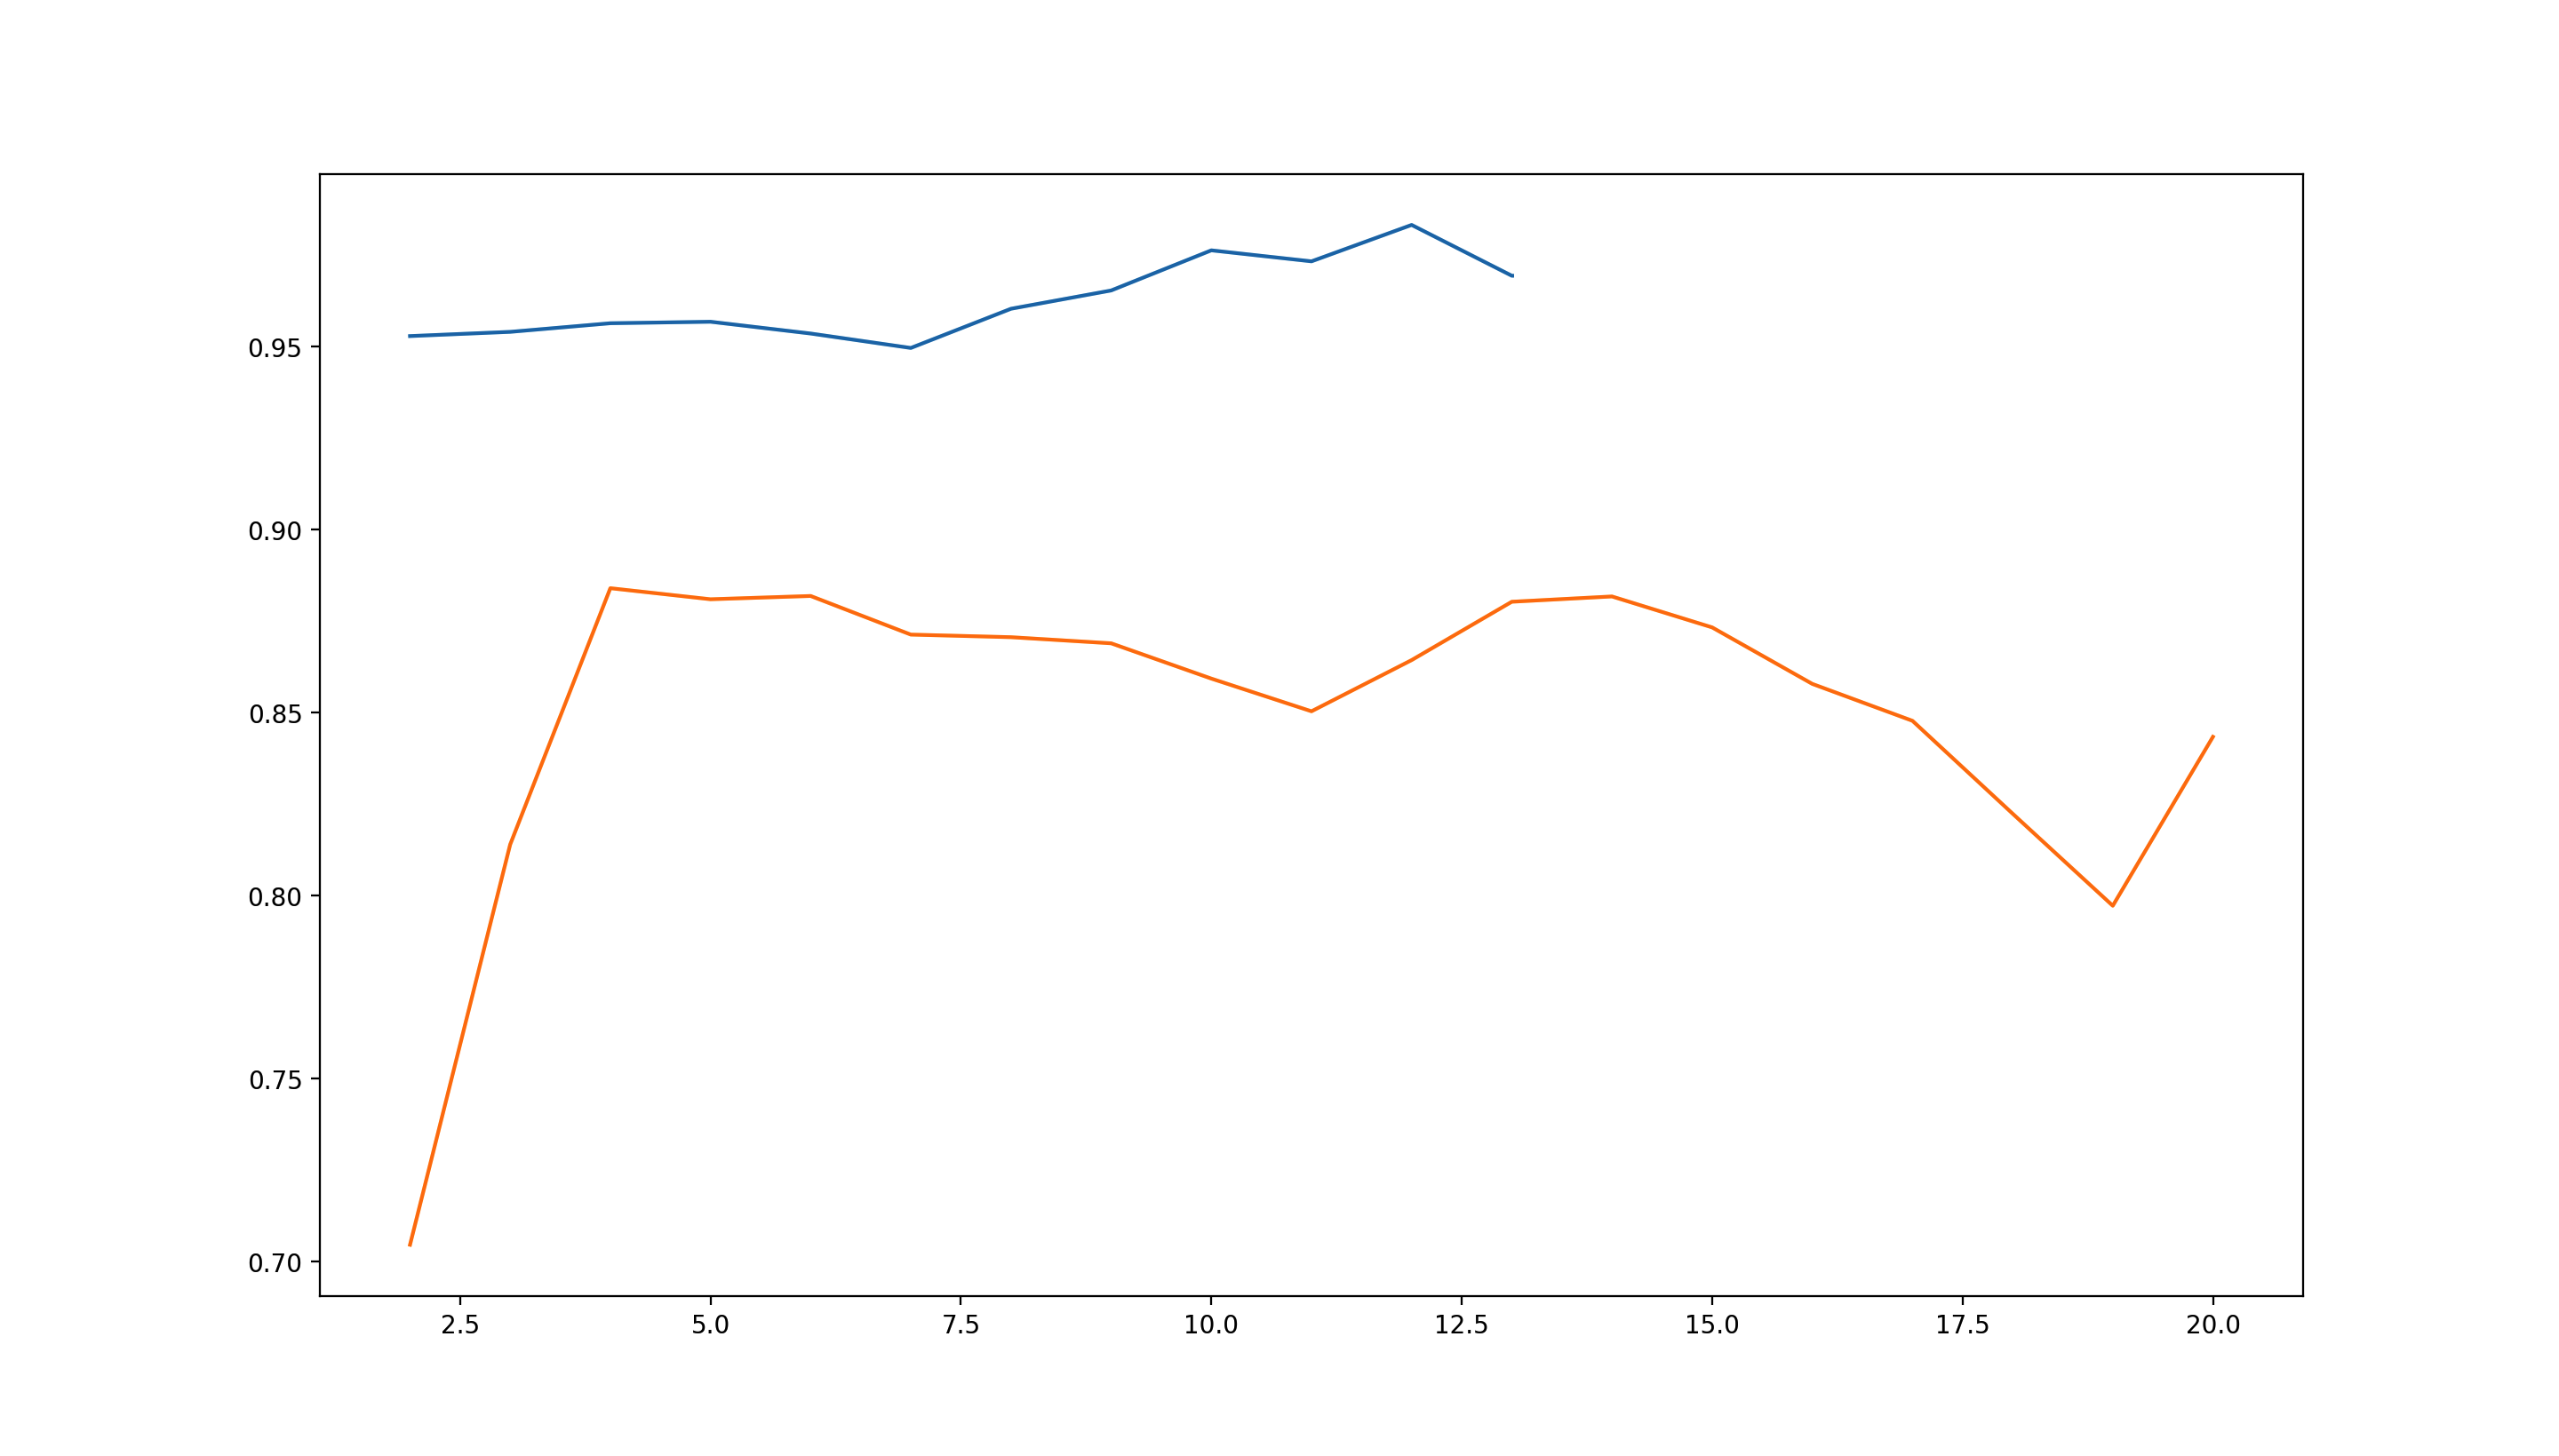
\includegraphics[width=\linewidth]{immagini/traintestrate.png}
	\caption{Accuracy in funzione del numero di giorni utilizzati come trainset. In blu è riportata l'accuracy del dataset A, in arancione quella del dataset B}
	\label{fig:traintestrate}
	\end{figure}
	
	% Timeslice da 60
	% In un caso abbiamo suddiviso in dataset nell'altro no
	
	\subsection{Analisi dei risultati}
	
	
	\subsubsection{Misure di qualità utilizzate}
	
	L'esecuzione dell'algoritmo di Viterbi su una sequenza di osservazioni, ha permesso di generare una sequenza di stati nascosti che, con una maggiore probabilità, ha portato alla realizzazione delle osservazioni date come input all'algoritmo.
	
	Una volta ottenuta la sequenza di stati frutto della previsione da parte dell'algoritmo di Viterbi, è stato possibile effettuare il confronto tra quest'ultima e la sequenza di stati reali, in modo da determinare la qualità dei risultati ottenuti.
	
	Per svolgere il controllo della qualità dei risultati sono stati testati i seguenti parametri:
	
	\begin{itemize}
		\item Accuracy
		\item Precision
		\item Recall
		\item F-Measure
	\end{itemize}

	Il test sulla Accuracy permette di trovare la percentuale di correttezza della sequenza di stati nascosti prevista. Di conseguenze, esprime, data una generica posizione i all'interno della sequenza di stati, se l'i-esimo stato nascosto previsto dall'algoritmo coincide con quello reale.
	
	Prima di descrivere le misure seguenti, è utile introdurre i termini vero positivo, vero negativo, falso positivo e falso negativo, i quali sono usati per confrontare la previsione dell'i-esimo stato nascosto rispetto il corretto stato alla posizione desiderata. Ad esempio:

	\begin{itemize}
		\item Vero positivo: l'i-esimo elemento corretto è sleeping e l'algoritmo ha predetto sleeping
		\item Vero negativo: l'i-esimo elemento corretto non è sleeping e l'algoritmo ha predetto non sleeping
		\item Falso positivo: l'i-esimo elemento corretto non è sleeping e l'algoritmo ha predetto sleeping
		\item Falso negativo: l'i-esimo elemento corretto è sleeping e l'algoritmo ha predetto non sleeping
	\end{itemize}	
	
	A questo punto è possibile introdurre le ultime misure di test; Precision e Recall verranno quindi definiti come segue:
	
	\begin{center}
		$ Precision = \dfrac{Veropositivo}{VeroPositivo + Falsopositivo} $
	\end{center}

	\begin{center}
		$ Recall = \dfrac{Veropositivo}{VeroPositivo + Falsonegativo} $
	\end{center}

	Infine, il test F-Measure permette di misurare l'accuratezza di un test, attraverso l'uso di Precision e Recall, ed è descritto dalla formula:
	
		\begin{center}
		$ F-Measure = 2 * \dfrac{Precision * Recall}{Precision + Recall} $
	\end{center}
	
	
	
	\subsubsection{Capacità predittiva del modello}
	
	% Abbiamo suddiviso testset e trainset
	% Abbiamo predetto sul testset
	
	\subsubsection{Predizione a lungo termine}
	
	% Abbiamo generato a cazzo
	% Abbiamo predetto
	
	
	\section{GUI}
	
	\section{Conclusioni}
\end{document}
